\documentclass[a4paper,11pt]{article}
\pdfoutput=1

\oddsidemargin 0.0in
\evensidemargin 0.0in
\textwidth 6.0in
\topmargin 0.2in
\footskip 20pt
\textheight 8.5in

\usepackage{hyperref,color,graphicx,braket,mathrsfs,amsmath,amssymb}
\hypersetup{colorlinks,%
	citecolor=blue,%
	linkcolor=blue,%
	filecolor=blue,%
	urlcolor=red}

\usepackage[numbers,sort]{natbib}
%\hypersetup{colorlinks, citecolor=blue, linkcolor=blue, filecolor=blue, urlcolor=red}

\begin{document} 
	
{\noindent\Large\textbf{DNNs in NEXT Analysis}}\\

\noindent This is a short note describing what problems are being addressed with DNNs in the NEXT analysis.

\section{Summary}\label{sec:summary}
\noindent We seek to accomplish three main tasks in NEXT analysis with DNNs.

\begin{enumerate}
	\item[1.] \textbf{Point reconstruction for energy calibration}: point-like calibration events (produced by Kr x-rays) are read out by the TPC.  The event must be reconstructed from its SiPM sensor map to a single point.  This point is then used as an index in a look-up table of energy correction factors.  The DNN must be trained with Monte Carlo events to reconstruct a single point from a set of $N \times N$ SiPMs, so that when Kr calibration data is taken, it can accurately reconstruct the point from an $N \times N$ subset of the tracking plane, and the energy measured by the PMTs can be recorded for that point. The correction table can then be constructed from this indexed table of energies.
	\item[2.] \textbf{Track reconstruction for energy correction}: full events with long tracks are read out from the TPC.  These tracks can then be sliced in the $z$ (time) direction and a pixelized $xy$ projection reconstructed from the set of SiPM sensor responses corresponding to light arriving in each time slice.  The energy correction for each pixel in the projection can be determined by indexing the table constructed in step 1, and the total energy correction for the slice can therefore be computed.  The DNN must be trained on Monte-Carlo-generated slices, preferably taken from Monte Carlo tracks of energies similar to those of the kinds of events we will be attempting to reconstruct.
	\item[3.] \textbf{Event classification}: the corrected slice energies and SiPM response maps for each slice must then be passed to a DNN for classification as signal or background. The net should be trained on Monte Carlo events prepared in the same way as real events.  As in step 1, an SiPM response map size should be chosen such that nearly all event sizes are contained without making use of too many unnecessary inputs.
\end{enumerate}

\noindent To conduct a complete study, for each of the above tasks we should have: 

\begin{enumerate}
	\item[-] \textbf{a suitable DNN}: this is chosen by studying several net architectures and identifying the best net for the task.
	\item[-] \textbf{an example application}: consisting of a simulated dataset for training (which will be used in real applications) and a simulated test set, demonstrating the performance of the net using Monte Carlo data. Note that in the interest of applying the same analysis to both real data and Monte Carlo, this would mean that the DNN has been properly integrated into the main analysis.
	\item[-] \textbf{a comparison to a classical analysis}: to demonstrate any potential advantages of the DNN-based approach.  Ideally we want to run a parallel classical analysis when analyzing real data in order to check whether the DNN is performing properly. 
\end{enumerate}

\noindent\textbf{Other notes:}

\begin{enumerate}
	\item[-] In all cases, the DNN must be trained with events for which we know the \emph{true} answer.  This means, for example, that in the track reconstruction step we need to have more than the SiPM map of Monte-Carlo generated responses - we also need to have a pixelized $xy$ projection for each slice to be given as the true information in training the DNN.  
	\item[-] The decision must also be made as to what data to use to train the net.  Consider the following: we can run toy models (MAGBOX, single-points with light parameterization, etc.) relatively quickly, while running events through the full MC chain is often much more time consuming.  Before attempting to generate many full-MC events, we should \textbf{train using toy data and then test using full-MC data}.  Say we train the classifier with 400k MAGBOX events and validate it on 5000 MAGBOX events, and then we get the same results in evaluating 5000 full-MC events.  This probably means we don't need to run 400k full-MC events to use for training - we should do this check first.  We therefore have to consider what effects to model in the toy (and whether or not they can be modeled efficiently or correctly in the toy).  For example, do we want to train the classification net using SiPM response maps with or without simulated SiPM noise included?  
	\item[-] How should the application of all of these nets be included in the analysis?  Note that we also must implement the training step for each net in code which can be easily re-run, and we must be able to generate more events when necessary.  One option is to have a ``city'' for the application of each net and to keep the training code outside the main Invisible Cities analysis flow but still readily accessible.  Note that task 1 (point reconstruction for calibration) may be kept outside of the main analysis flow entirely as it is used only in creating the energy correction table.
\end{enumerate}

\section{Point reconstruction}\label{sec:ptreconstruction}
\subsection{Training}
\noindent The current idea is to choose random points over an $N \times N$ grid of SiPM planes and generate SiPM responses for all sensors in the plane using the S2 parameterization.  Note that $N$ must be chosen to minimize the number of inputs while still capturing the relevant amount of SiPM response.  Knowing the true location from which the light was generated, the net can be trained over many such events.  Since the energy correction table will attempt to provide a correction factor for each $(x,y)$ location, the DNN will be constructed to yield a single $(x,y)$ pair for an input SiPM map.  

\subsubsection{Questions}
\begin{enumerate}
	\item[-] Do we include SiPM noise in the training events?
	\item[-] Do we use ``toy'' events generated using the SiPM parameterization or will we use full-MC Kr events?
\end{enumerate}

\subsection{Application}
\noindent The $N \times N$ subset of SiPMs containing the responses generated by the EL light produced by a real (or full-MC) Kr x-ray must be isolated from all of the sensors in the tracking plane.  We should attempt to centralize the point (the hottest SiPM should be near the center of the $N \times N$ subsection) unless the event occurred near the edge of the tracking plane, making this impossible.  Either way, the DNN should be prepared to properly reconstruct non-centralized points.

\section{Track reconstruction}\label{sec:trkreconstruction}
\subsection{Training}
For now, the current training procedure is:

\begin{enumerate}
	\item[1.] Generate a large number of MAGBOX events (signal and background).
	\item[2.] Voxelize the MC truth.  The voxels need not be connected.
	\item[3.] Slice the events in slices of width $w$ using the voxelized MC truth, including all voxels in the $xy$ plane with $z$ in the range of the slice $(z_i, z_i + w)$.  Each slice is then a 2D grid (with pixel dimensions equal to those of the voxel $xy$ dimensions) containing some energy.  If any slice in the event has an $xy$ range greater than some value, or if more $z$ slices than some limit are present, do not include any slices from the event in the training set.
	\item[4.] For each slice, normalize the total energy to 1, and for each pixel in the slice containing nonzero energy, cast EL light on an $M \times M$ SiPM plane (M to be chosen appropriately, currently $M = 20$) using the S2 parameterization.  This SiPM map along with the true slice information constitutes the input and truth for a single training event.
	\item[5.] Train the net on the constructed slices.  Using a softmax output layer, the reconstructed projection will provide a normalized image of the track.
\end{enumerate}

\noindent An example of a training event (truth, SiPM map, and reconstructed slice) is shown in figure \ref{fig:slice_train}.

\begin{figure}[!htb]
	\centering
	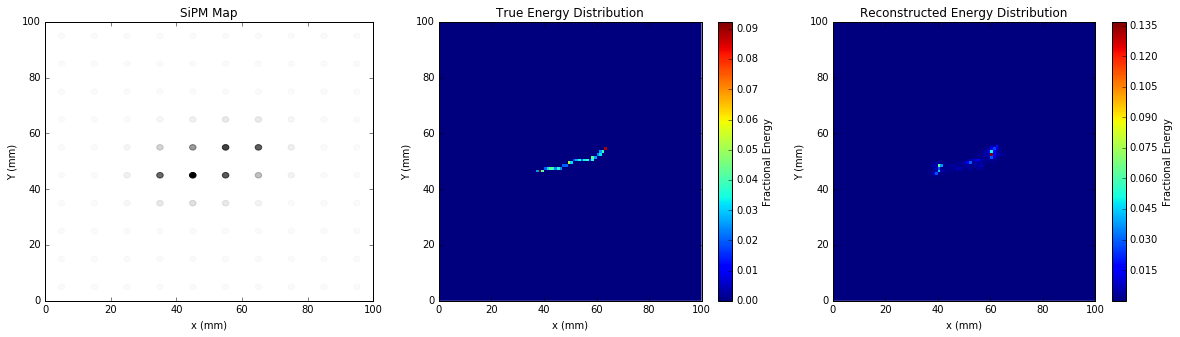
\includegraphics[scale=0.41]{fig/reconst_example_evt1.png}
	\caption{\label{fig:slice_train}Example of reconstruction of a single slice. The normalized SiPM map (left) produced by the true energy distribution (middle), as reconstructed by a simple CNN (right).}
\end{figure}

\section{Event classification}\label{sec:evtclassification}
\noindent 

%\bibliography{dnnext}

\end{document}